\section{Première séance}

\subsection{Paramètres à prendre en compte}
\begin{itemize}
    \item La géométrie de la pièce dont l'épaisseur peut être variable.
    \item La géométrie du poinçon et de la matrice de pliage.
    \item Les caractéristiques mécaniques du matériau en traction et en compression en intégrant  les phénomènes de déformation plastique et retour élastique.
\end{itemize}
\subsection{Résultats à fournir}
\begin{itemize}
    \item La simulation du mouvement de la pièce avec la possibilité d'extraire la trajectoire de n'importe quel point de la pièce.
    \item Le retour élastique de la pièce et les corrections géométriques à appliquer au poinçon et à la matrice initial afin d'obtenir la pièce exacte.
    \item Toutes les explications nécessaires concernant le modèle et les algorithmes mis en œuvre afin de permettre une intégration future dans TopSolid.
\end{itemize}
\begin{figure}[H]
    \begin{center}
        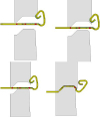
\includegraphics[width=0.5\textwidth]{img/img1.jpg}
        \caption{Exemple de pliage}
        \label{img1}
    \end{center}
\end{figure}
\subsection{Revue du sujet}
\begin{itemize}
    \item Définition des éléments géométriques:
    \begin{itemize}
        \item Pièces (épaisseur variable?).
        \item Poinçons.
        \item Matrices.
    \end{itemize}
    \item Phénomènes physiques à prendre en compte:
    \begin{itemize}
        \item Élasticité (et retour élastique).
        \item Plasticité.
        \item Frottements.
    \end{itemize}
    \item Résultats désirés (utilisateur):
    \begin{itemize}
        \item Étapes de simulation du mouvement.
        \item Trajectoires et points clés.
        \item Contraintes, déformations, amincissements.
        \item Corrections à appliquer sur les poinçons et matrices pour obtenir la pièce finale.
    \end{itemize}
    Résultats désirés (MS):
    \begin{itemize}
        \item Modèles utilisés et hypothèses.
        \item Méthodes et algorithmes.
        \item Exemples de validation sur la base d'exemples proposés par MS.
    \end{itemize}
\end{itemize}
    
